\documentclass[11pt,letterpaper]{article}
\usepackage[margin=0.82in]{geometry}
\usepackage{amsmath,amssymb,booktabs,graphicx,xcolor,hyperref,fancyhdr,enumitem,array}
\usepackage[T1]{fontenc}
\usepackage{lmodern,microtype,titlesec,caption,float}
\titleformat{\section}{\large\bfseries}{\thesection}{0.65em}{}
\titleformat{\subsection}{\normalsize\bfseries}{\thesubsection}{0.65em}{}
\titlespacing*{\section}{0pt}{13pt plus 2pt}{4pt}
\titlespacing*{\subsection}{0pt}{9pt plus 1pt}{2pt}
\captionsetup{font=small,labelfont=bf,labelsep=period,justification=raggedright,singlelinecheck=false,skip=5pt}
\setlength{\intextsep}{9pt plus 2pt minus 2pt}
\renewcommand{\arraystretch}{1.10}
\raggedbottom
\clubpenalty=10000
\widowpenalty=10000
\definecolor{navy}{HTML}{18364A}
\hypersetup{colorlinks=true,urlcolor=navy,linkcolor=navy,citecolor=navy}
\setlength{\emergencystretch}{3em}
\setlength{\parindent}{0pt}\setlength{\parskip}{5pt}
\setlist[itemize]{nosep,leftmargin=*}
\pagestyle{fancy}\fancyhf{}\fancyhead[L]{\small CISC 473 | P08 | Group 04}\fancyhead[R]{\small Final Report}\fancyfoot[C]{\thepage}
\setlength{\headheight}{14pt}
\newcommand{\psection}[1]{\section{#1}}
\begin{document}
\begin{center}
{\LARGE\bfseries Where to Adapt BART?}\\[5pt]
{\large A Controlled LoRA Placement Study for News Summarization}\\[7pt]
Choo Wen Bin (20630085) \quad Nai Junn Rong (20630086)\\
Group 04 \quad CISC 473, Fall 2026\\
\url{https://github.com/wenbin05/DeepLearningP08}
\end{center}
\begin{abstract}
We study whether LoRA placement changes BART-base summarization under an equal trainable-parameter budget. Encoder self-attention, decoder self-attention, and cross-attention each receive 147,456 trainable parameters. We train on 1,024 CNN/DailyMail examples for 96 updates and evaluate three seeds on 128 held-out examples from each of CNN/DailyMail and XSum. Cross-attention attains the highest CNN/DailyMail ROUGE-1 among the matched placements, 38.56 $\pm$ 0.42, compared with 37.75 $\pm$ 0.29 for encoder and 37.50 $\pm$ 0.22 for decoder adaptation. Unadapted BART scores 38.61. Full fine-tuning, evaluated as a memory-adjusted reference, reaches 40.06 $\pm$ 0.62. Rank and projection ablations show that adding parameters does not monotonically improve ROUGE. A ten-participant study yields low agreement (Fleiss' $\kappa=0.044$), so its model-level ratings are descriptive. These results support a bounded placement comparison, but do not establish a factuality winner or performance on the full benchmarks.
\end{abstract}
\section{Introduction}
Abstractive summarization requires both selecting information and generating text supported by the source. BART combines a bidirectional encoder with an autoregressive decoder~\cite{bart}. Full fine-tuning updates the entire model, whereas LoRA trains low-rank weight updates while freezing the backbone~\cite{lora}. This changes the adaptation budget, but it does not determine where that budget is most useful.

We ask: \textit{When trainable capacity and training conditions are fixed, how does LoRA placement affect in-domain quality and transfer?} Encoder self-attention represents the source, decoder self-attention represents the generated prefix, and cross-attention connects decoder states to the source. Their different computational roles motivate a controlled comparison; they do not, by themselves, predict which placement will win.

Our contributions are:
\begin{itemize}
\item An exact-budget comparison of three attention regions, each with 147,456 trainable parameters, using identical main-study settings.
\item A completed 39-run matrix spanning baselines, ranks and projections, with 78 held-out test evaluations and saved predictions for score verification.
\item A descriptive human evaluation and a concrete failure analysis that separate lexical overlap from factual consistency.
\end{itemize}
The final study extends the midterm's single-seed validation pilot. Its results use held-out test subsets and are not pooled with pilot measurements. The limited data and training budget are part of the experimental scope, rather than evidence of benchmark-scale reproduction.

\section{Related Work and Method}
\subsection{Generation, adaptation and evaluation}
BART's denoising pretraining provides the encoder--decoder backbone for this study~\cite{bart}. LoRA and Prefix-Tuning offer two ways to adapt frozen models~\cite{lora,prefix}: low-rank weight updates and learned continuous conditioning, respectively. Comparing them under a short training schedule measures behavior under that schedule, not the best attainable result of either method.

The unified PEFT framework connects several adaptation mechanisms and motivates examining where trainable capacity enters a Transformer~\cite{unified}. AdaLoRA allocates rank according to estimated parameter importance~\cite{adalora}; DyLoRA studies flexible ranks~\cite{dylora}; WeightLoRA examines adapter selection~\cite{weightlora}. Our experiment instead fixes explicit architectural regions. It does not implement these adaptive-allocation methods, and it does not claim that an architectural ablation is a new adaptation algorithm.

Factuality is a separate evaluation problem. FactCC evaluates whether generated claims are supported by the source~\cite{factcc}. ROUGE measures lexical overlap and can reward a summary that retains many source words while changing a critical fact. This motivates our human assessment and source-grounded examples. We do not report FactCC scores because that classifier was not run.
\subsection{Architecture and exact adapter budget}
BART-base has six encoder layers, six decoder layers and hidden dimension 768. For a frozen projection $W_0\in\mathbb{R}^{768\times768}$, LoRA learns
\[
W=W_0+\frac{\alpha}{r}BA,\qquad
A\in\mathbb{R}^{r\times768},\quad B\in\mathbb{R}^{768\times r}.
\]
The main comparison uses $r=8$, $\alpha=16$, dropout 0.05, query and value projections, and no trainable bias. Each region has six attention blocks and two target projections. Its budget is therefore
\[
6\times2\times8\times(768+768)=147{,}456.
\]
This is 0.10565\% of the model's 139,567,872 total parameters including adapters. Module-name checks verify the actual target set and live trainable count; the comparison does not rely on configuration names alone.
\subsection{Objective and comparison methods}
We minimize teacher-forced token cross-entropy,
\[
\mathcal{L}=-\frac{1}{N}\sum_{t\in\text{non-padding targets}}
\log p_\theta(y_t\mid y_{<t},x),
\]
where $N$ counts non-padding target tokens in the loss calculation. Labels use $-100$ for ignored padding. Generation is evaluated separately from this training objective.

Baselines are unadapted BART, all-attention QV LoRA at rank eight, Prefix-Tuning with 20 virtual tokens and no prefix projection, and full fine-tuning. All-attention LoRA reaches all three attention regions. Prefix-Tuning uses the PEFT sequence-to-sequence implementation; it is not a placement-matched control.

\section{Experimental Protocol}
\subsection{Data and preprocessing}
The official CNN/DailyMail 3.0.0 splits~\cite{data} supply 1,024 training, 64 validation and 128 test examples. A separate 128-example XSum test subset measures transfer without XSum training or tuning. Subsets are selected with fixed data seed 42, independently of training seeds 42, 123 and 999. Saved IDs and hashes make membership comparable across configurations. Training order and adapter initialization vary with the training seed.

The BART tokenizer truncates sources to 1,024 tokens and training targets to 128 tokens. Dynamic padding is used. ROUGE compares generated text with \textit{untruncated original reference summaries}; teacher-forced loss uses the tokenized targets. Long-source truncation can remove relevant evidence, and this study does not measure the frequency of that event.
\subsection{Training and decoding}
All adapted runs use three epochs, 96 optimizer updates, an effective batch size of 32 and ten warmup steps. AdamW uses weight decay 0.01, $\beta_1=0.9$, $\beta_2=0.999$, $\epsilon=10^{-8}$, gradient clipping at 1.0 and a linear learning-rate schedule. LoRA and Prefix-Tuning use learning rate $3\times10^{-4}$; full fine-tuning uses $3\times10^{-5}$. Checkpoints are taken from the final epoch/update, rather than selected by test scores. Epoch validation monitors the run; it does not choose the final model.

Deterministic beam search uses four beams, maximum length 128, minimum length 56, length penalty 2.0 and a no-repeat trigram constraint. These settings are shared across datasets and methods. In particular, they are not adapted to XSum's shorter reference style, which limits interpretation of transfer quality.
\subsection{Compute and fairness boundary}
Runs use CPU execution with two compute threads and an 8 GiB memory limit, without mixed precision. The main placements, other LoRA runs and Prefix-Tuning use microbatch two and accumulation 16. Full fine-tuning exhausted memory during its first attempt. Completed full-FT runs restart from pretrained weights with microbatch one and accumulation 32, plus an allocator arena limit of two. The failed run is archived and excluded.

Equal effective batch size preserves nominal examples per optimizer update; it does not guarantee identical dropout draws or token weighting. Full FT also uses a different learning rate. We therefore label it a \textit{memory-adjusted reference baseline}. The guide's matched-compute objective is only partially met: data exposure and update counts match, but FLOPs and wall-clock time are not equalized. The three main placements retain the same microbatch, optimizer and data settings.
\subsection{Metrics and uncertainty}
ROUGE-1, ROUGE-2 and ROUGE-L are stemmed per-example F1 scores~\cite{rouge}, macro-averaged and multiplied by 100 using pinned Hugging Face Evaluate ROUGE. ROUGE-L is not ROUGE-Lsum. We report mean and sample standard deviation over three training seeds, with denominator $n-1$. These deviations measure seed variability on fixed test examples, not population confidence intervals. Unadapted outputs are identical across the three seed labels, so their zero deviation does not represent independent trained models. No significance test is claimed.

\section{Held-Out Results}
\subsection{CNN/DailyMail}
\begin{table}[H]
\centering
\small
\begin{tabular}{lrrr}\toprule Configuration & ROUGE-1 & ROUGE-2 & ROUGE-L\\\midrule
Unadapted & 38.61 $\pm$ 0.00 & 16.91 $\pm$ 0.00 & 24.29 $\pm$ 0.00\\
Encoder & 37.75 $\pm$ 0.29 & 16.48 $\pm$ 0.15 & 23.29 $\pm$ 0.23\\
Decoder & 37.50 $\pm$ 0.22 & 16.17 $\pm$ 0.16 & 23.53 $\pm$ 0.18\\
Cross-attention & 38.56 $\pm$ 0.42 & 16.78 $\pm$ 0.42 & 24.42 $\pm$ 0.51\\
All-attention & 38.92 $\pm$ 0.08 & 16.84 $\pm$ 0.15 & 25.08 $\pm$ 0.24\\
Prefix & 15.05 $\pm$ 3.03 & 2.41 $\pm$ 0.97 & 10.63 $\pm$ 1.42\\
Full FT* & 40.06 $\pm$ 0.62 & 17.21 $\pm$ 0.33 & 26.34 $\pm$ 0.39\\
\bottomrule\end{tabular}
\caption{CNN/DailyMail test subset (128 examples). Mean $\pm$ sample SD across three seeds. *Full FT uses the memory-adjusted protocol.}
\end{table}

Cross-attention has the highest mean ROUGE-1, ROUGE-2 and ROUGE-L among the three isolated placements. Its ROUGE-1 exceeds encoder by 0.81 points and decoder by 1.06 points. However, it is 0.05 points below unadapted BART on ROUGE-1 and 0.13 points below it on ROUGE-2. Cross-attention's ROUGE-L is 0.14 points higher. Thus the placement ranking is clearer than the case for improvement over the unadapted model. All-attention QV LoRA has a higher ROUGE-1 mean, but also uses three times the adapter budget.

Full fine-tuning has the highest mean scores in this baseline table. Prefix-Tuning performs poorly in this implementation and short-budget setting. Its CNN/DailyMail ROUGE-1 is 15.05 $\pm$ 3.03 and teacher-forced test loss is 7.10 $\pm$ 0.34. The evidence supports an unsuccessful baseline configuration, not a general rejection of Prefix-Tuning. More training and method-specific optimization would be needed to distinguish those explanations.
\subsection{CNN/DailyMail-to-XSum transfer}
\begin{table}[H]
\centering
\small
\begin{tabular}{lrrr}\toprule Configuration & ROUGE-1 & ROUGE-2 & ROUGE-L\\\midrule
Unadapted & 16.84 $\pm$ 0.00 & 2.62 $\pm$ 0.00 & 10.51 $\pm$ 0.00\\
Encoder & 16.68 $\pm$ 0.16 & 2.85 $\pm$ 0.10 & 10.60 $\pm$ 0.10\\
Decoder & 16.85 $\pm$ 0.11 & 2.74 $\pm$ 0.08 & 10.67 $\pm$ 0.08\\
Cross-attention & 16.87 $\pm$ 0.02 & 2.74 $\pm$ 0.02 & 10.73 $\pm$ 0.03\\
All-attention & 17.16 $\pm$ 0.09 & 3.01 $\pm$ 0.03 & 11.00 $\pm$ 0.06\\
Prefix & 9.75 $\pm$ 1.71 & 1.26 $\pm$ 0.50 & 7.76 $\pm$ 1.07\\
Full FT* & 19.17 $\pm$ 0.23 & 3.16 $\pm$ 0.21 & 12.59 $\pm$ 0.14\\
\bottomrule\end{tabular}
\caption{XSum test subset (128 examples), evaluated without further tuning. The same decoding policy is retained.}
\end{table}

The isolated placements' ROUGE-1 means are close: 16.68 for encoder, 16.85 for decoder and 16.87 for cross-attention. Cross-attention exceeds decoder by only 0.02 points. Encoder has the highest ROUGE-2 of these three placements, so there is no uniform transfer ranking across metrics. Full FT reaches 19.17 ROUGE-1 and all-attention QV LoRA reaches 17.16. These results do not support the proposed expectation that PEFT necessarily transfers better than full fine-tuning. Dataset style, the fixed generation policy and limited training all remain relevant.

\section{Rank and Projection Ablations}
\begin{table}[H]
\centering
\small
\begin{tabular}{lrrr}\toprule All-attention configuration & Trainable & CNN R-1 & XSum R-1\\\midrule
QV, r=4 & 221,184 & 39.12 $\pm$ 0.46 & 17.24 $\pm$ 0.14\\
QV, r=8 & 442,368 & 38.92 $\pm$ 0.08 & 17.16 $\pm$ 0.09\\
QV, r=16 & 884,736 & 38.87 $\pm$ 0.36 & 17.17 $\pm$ 0.14\\
Q, r=8 & 221,184 & 38.10 $\pm$ 0.11 & 16.59 $\pm$ 0.10\\
K, r=8 & 221,184 & 38.65 $\pm$ 0.17 & 16.70 $\pm$ 0.07\\
V, r=8 & 221,184 & 39.08 $\pm$ 0.35 & 17.05 $\pm$ 0.07\\
QKVO, r=8 & 884,736 & 39.54 $\pm$ 0.32 & 17.85 $\pm$ 0.08\\
\bottomrule\end{tabular}
\caption{Rank and projection ablations. Q, K, V and O denote query, key, value and attention-output projections. All rows use three seeds; the full ROUGE tables appear in the appendix.}
\end{table}

\begin{figure}[H]
\centering
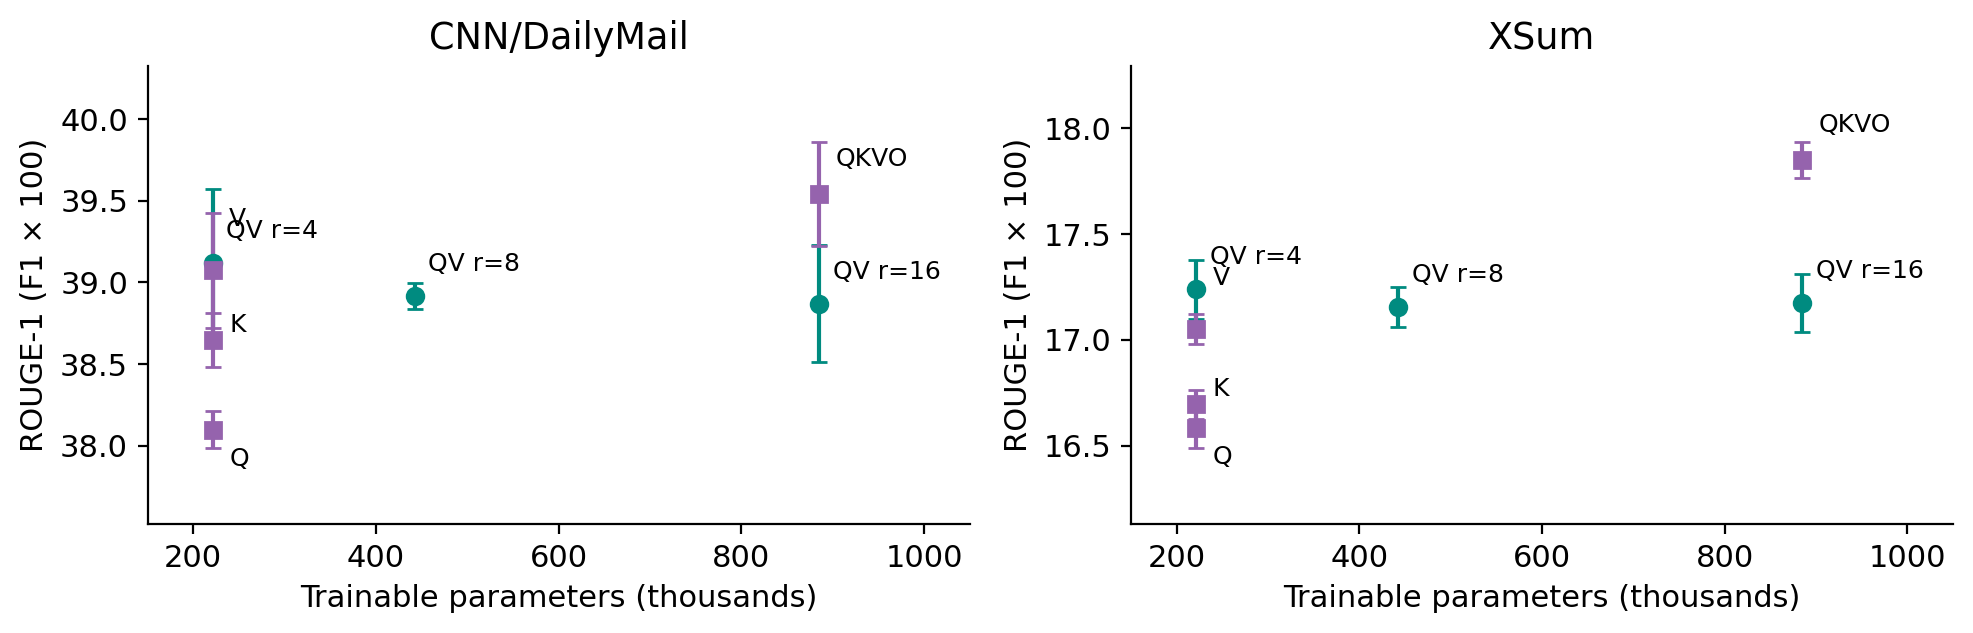
\includegraphics[width=\linewidth]{figures/ablations.png}
\caption{ROUGE-1 against trainable parameters. Error bars show seed SD. Vertical axes are restricted to the observed range to make differences visible; these are not confidence intervals. Green circles vary QV rank; purple squares vary projection targets at rank eight.}
\end{figure}

Increasing QV rank from four to eight to sixteen does not yield monotonic gains. CNN/DailyMail ROUGE-1 changes from 39.12 to 38.92 to 38.87; XSum changes from 17.24 to 17.16 to 17.17. Alpha is fixed at 16, so the update multiplier $\alpha/r$ changes from four to two to one. This is an ablation of the implemented rank configurations, not a test that isolates rank from scaling.

Q-only, K-only and V-only each use 221,184 parameters at rank eight. V-only has the highest ROUGE-1 mean among these single-projection variants on both datasets, while K-only has the highest CNN/DailyMail ROUGE-2. QKVO has the highest ROUGE-1 among the LoRA configurations evaluated, but requires 884,736 trainable parameters. At the same parameter count, QKVO rank eight exceeds QV rank sixteen in ROUGE-1 on both datasets. That comparison changes projection coverage, rank and scaling together; it cannot identify which factor causes the difference.

The ablations suggest that parameter count alone is insufficient to predict quality within this setup. They do not establish an optimal rank or target set for larger training datasets, other learning rates or other decoding policies. The test set was used to report the predefined matrix, not to retrain a selected winner.

\section{Human Factual-Consistency Evaluation}
\subsection{Design and provenance}
Ten participants each rated the same twenty generated summaries: five shared CNN/DailyMail articles times four configurations (unadapted, encoder, decoder and cross-attention), using training seed 42. Summary order was randomized separately for each packet, and model identities were hidden during rating. Shared items allow agreement to be measured; presenting different orders does not create different evaluation examples.

Participants compared each summary with its article and selected consistent, inconsistent or uncertain, with space for supporting explanations. The project team reports that participants completed the ratings independently. The final submitted response files are preserved unchanged. The analysis uses those human responses, not an AI evaluator substituted for participants.
\begin{table}[H]
\centering
\small
\begin{tabular}{lrrr}\toprule Configuration & Consistent & Inconsistent & Consistent share\\\midrule
Cross-attention &29&21&58\%\\
Unadapted &27&23&54\%\\
Decoder &23&27&46\%\\
Encoder &19&31&38\%\\\bottomrule\end{tabular}
\caption{Each configuration receives 50 ratings over five summaries. There are no uncertain responses. Across all configurations, 98 of 200 ratings are consistent.}
\end{table}
\begin{figure}[H]
\centering
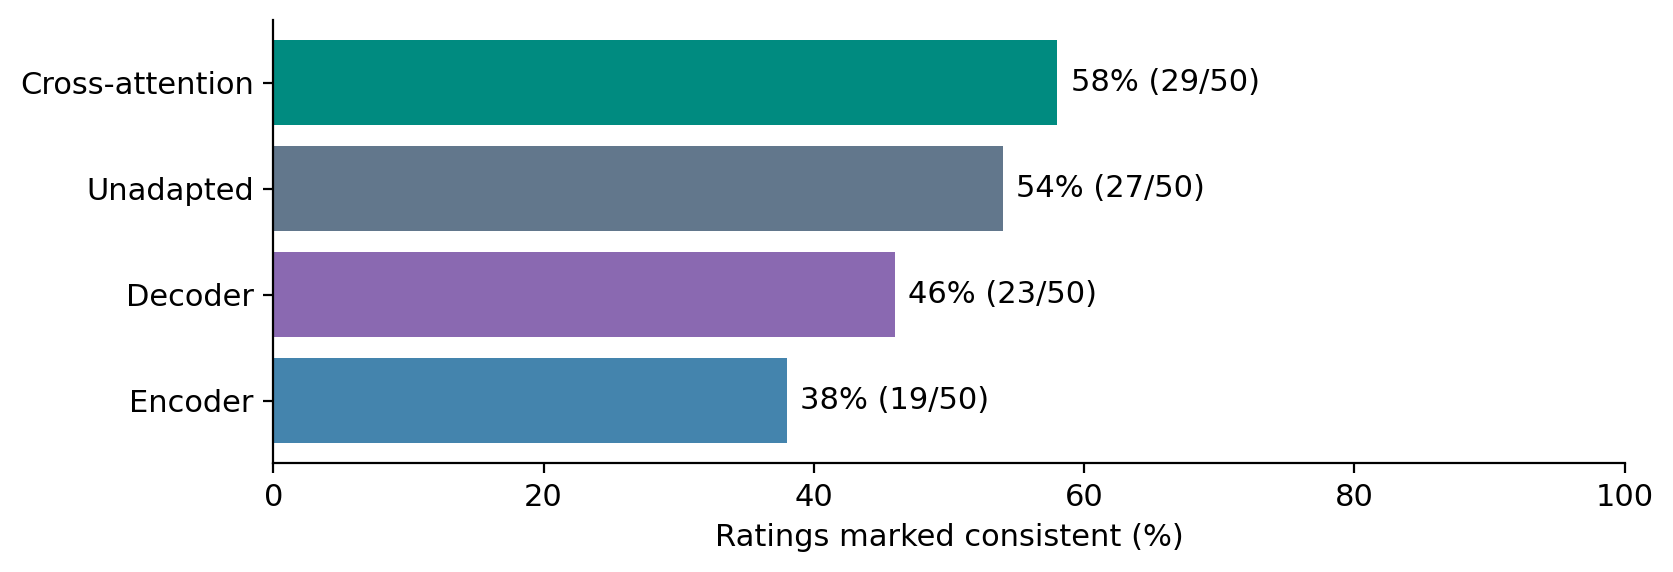
\includegraphics[width=.78\linewidth]{figures/human.png}
\caption{Descriptive proportions of ratings marked consistent. These are not estimates from fifty independent articles per configuration.}
\end{figure}
\subsection{Agreement and interpretation}
Mean pairwise agreement is 0.5222 and Fleiss' $\kappa$ is 0.0441, indicating little agreement beyond chance under this coding. Some explanations treat missing details, name variations or stylistic issues as inconsistencies, which can broaden the intended factuality criterion. We retain those judgments rather than recoding them to improve the ranking.

Cross-attention has the highest consistent-rating proportion, but only two more consistent judgments than unadapted BART. Five articles, one training seed and low agreement are insufficient to establish a reliable factuality advantage. The 200 responses share articles, outputs and participants; treating them as 200 independent examples would overstate the evidence. Full FT, Prefix-Tuning and the additional ablations were not included in this study.

A stronger follow-up would use a brief calibration task, distinguish unsupported claims from omissions, sample more articles and report agreement before interpreting model-level differences. It should preserve independent judgments and preregister any adjudication procedure.

\section{Failure Analysis and Training Cost}
\subsection{A source-grounded failure}
One sampled article describes taekwondo athlete Aaron Cook. It states that he is 24, has received a Moldovan passport and plans to represent Moldova. The encoder-LoRA output for seed 42 instead contains these excerpts:
\begin{quote}\small
``The 31-year-old has been granted citizenship by Moldova.''\\
``The British taekwarondo star has been denied citizenship by the Republic of Moldova.''
\end{quote}
The age is unsupported by the article, and the citizenship statement contradicts both the source and an earlier sentence in the generated summary. The generated quotation also replaces ``representing the Republic of Moldova'' with ``representing my country of birth,'' changing its meaning. All ten participants rated this output (S11) inconsistent.

This is a selected illustrative case, not a measured prevalence estimate. It shows why copying many source words does not ensure support for every proposition. The error includes a numeric change, a polarity reversal and inconsistent attribution. No attention-map or causal intervention was performed, so it cannot be attributed specifically to an internal attention mechanism. The source ID and unedited generated text are preserved in the evidence bundle.
\subsection{Observed training-loop cost}
\begin{table}[H]
\centering
\small
\begin{tabular}{lrrr}\toprule Configuration & Trainable & Fraction (\%) & Loop hours\\\midrule
Unadapted & 0 & 0.00000 & 0.00 $\pm$ 0.00\\
Encoder & 147,456 & 0.10565 & 2.31 $\pm$ 0.07\\
Decoder & 147,456 & 0.10565 & 1.42 $\pm$ 0.02\\
Cross-attention & 147,456 & 0.10565 & 1.39 $\pm$ 0.03\\
All-attention & 442,368 & 0.31629 & 2.35 $\pm$ 0.03\\
Prefix & 184,320 & 0.13203 & 1.44 $\pm$ 0.04\\
Full FT* & 139,420,416 & 100.00000 & 2.39 $\pm$ 0.01\\
\bottomrule\end{tabular}
\caption{Mean $\pm$ sample SD of successful training-loop wall times. Fractions use total model parameters including adapters. Loop time includes epoch validation and checkpoint saving, but excludes initial model/data preparation and the separately executed final validation and test prediction passes. The failed full-FT attempt is excluded.}
\end{table}

Equal adapter counts do not imply equal runtime. Encoder-only adaptation takes about 2.31 hours per training loop, compared with 1.39 for cross-attention and 1.42 for decoder-only adaptation. Backpropagation paths and sequence lengths offer plausible explanations, but these measurements do not isolate their contributions. Unadapted BART has no training loop; its generation cost is not zero.

The roughly 0.106\% trainable fraction of each isolated placement represents a reduction in optimized parameters, not a corresponding reduction in total model memory or total computation. Frozen weights and activations still occupy memory. The full-FT memory failure makes this distinction concrete. No peak-memory ranking across configurations is claimed because a consistent full-run memory benchmark was not collected.

\section{Discussion, Limitations and Conclusion}
\subsection{What the study supports}
Under the shared short-budget protocol, cross-attention is the strongest isolated placement on CNN/DailyMail by the three reported ROUGE means. Holding the target projections, rank, parameter count and training settings fixed makes this comparison more interpretable than comparing adapters with different capacity. It is still a finite experiment on one backbone and one training subset; the measurements do not establish a universal architectural preference.

The broader comparisons change the interpretation. Cross-attention does not exceed unadapted BART on CNN/DailyMail ROUGE-1, and full fine-tuning has the highest mean ROUGE-1 on both test subsets. Better fitting under teacher forcing also need not improve decoded summaries: decoder adaptation has lower CNN/DailyMail test loss than cross-attention (2.70 versus 2.78), yet lower ROUGE-1. Training loss and generation quality answer different questions.
\subsection{Limits and deviations from the initial plan}
The study completes its declared CPU matrix, including required baseline types, three seeds, rank/projection ablations, cross-domain evaluation and the human study. It does not reproduce published scores or evaluate the full test splits. Training uses 1,024 examples instead of the guide's larger suggested subset. The 64-example validation and 128-example test subsets limit generalization, and seed SD does not capture dataset-sampling uncertainty.

Full FT is an explicitly adjusted baseline, and the experiment does not equate FLOPs or wall time across methods. Minimum generation length 56 may be unsuitable for some XSum summaries. Alpha/r changes during rank ablation. Prefix-Tuning was not tuned separately beyond the shared PEFT settings. Human judgments cover only five articles and show low agreement. The qualitative example is selected and does not estimate an overall error rate. These limits prevent claims of benchmark superiority, statistical significance or improved factual reliability.
\subsection{Conclusion and next experiment}
The main result is a controlled placement comparison, not a new summarization model. Cross-attention uses the same 147,456 trainable parameters as the two isolated self-attention variants and achieves higher in-domain ROUGE means, while the unadapted baseline remains competitive. Wider projection coverage produces stronger LoRA ROUGE-1 means at a larger budget. Human evidence remains inconclusive.

A concrete next experiment would repeat the three matched placements on a larger preregistered training subset, retain the same examples and decoding within each comparison, and use paired article-level uncertainty estimates. A separate XSum decoding study should vary length constraints on validation data before evaluating a new held-out test set.
\subsection{Contributions and AI usage}
Choo Wen Bin and Nai Junn Rong contributed equally (50\% each).

We used OpenAI Codex for code implementation and the first report draft, with the academic-humanizer skill for writing feedback. Codex also helped run and check the experiments and prepare the analysis, figures and presentation.

\clearpage
\begin{thebibliography}{10}
\bibitem{bart} M. Lewis et al. BART: Denoising Sequence-to-Sequence Pre-training for Natural Language Generation, Translation, and Comprehension. ACL, pp. 7871--7880, 2020.
\bibitem{lora} E. J. Hu et al. LoRA: Low-Rank Adaptation of Large Language Models. ICLR, 2022. arXiv:2106.09685.
\bibitem{prefix} X. L. Li and P. Liang. Prefix-Tuning: Optimizing Continuous Prompts for Generation. ACL-IJCNLP, pp. 4582--4597, 2021.
\bibitem{adalora} Q. Zhang et al. Adaptive Budget Allocation for Parameter-Efficient Fine-Tuning. ICLR, 2023. arXiv:2303.10512.
\bibitem{unified} J. He et al. Towards a Unified View of Parameter-Efficient Transfer Learning. ICLR, 2022. arXiv:2110.04366.
\bibitem{dylora} M. Valipour et al. DyLoRA: Parameter-Efficient Tuning of Pre-trained Models using Dynamic Search-Free Low-Rank Adaptation. EACL, pp. 3274--3287, 2023.
\bibitem{weightlora} A. Veprikov et al. WeightLoRA: Keep Only Necessary Adapters. ACL, pp. 12419--12437, 2026. Bibliographic information retained from the supplied midterm report.
\bibitem{factcc} W. Kryscinski et al. Evaluating the Factual Consistency of Abstractive Text Summarization. EMNLP, pp. 9332--9346, 2020.
\bibitem{rouge} C.-Y. Lin. ROUGE: A Package for Automatic Evaluation of Summaries. Text Summarization Branches Out, pp. 74--81, 2004.
\bibitem{data} Hugging Face dataset repositories: \texttt{abisee/cnn\_dailymail} (3.0.0) and \texttt{EdinburghNLP/xsum}. Exact revisions are recorded in Appendix B.
\end{thebibliography}
\appendix
\section{Complete Test Tables}
All values below use the same metric protocol described in Section 3. Trainable-parameter counts for all-attention variants appear in Table 3. No prefix or full-FT human judgments were collected.
\subsection{CNN/DailyMail}
\begin{center}\small
\begin{tabular}{lrrr}\toprule Configuration & ROUGE-1 & ROUGE-2 & ROUGE-L\\\midrule
All r4 QV & 39.12 $\pm$ 0.46 & 16.92 $\pm$ 0.57 & 25.10 $\pm$ 0.46\\
All r8 K & 38.65 $\pm$ 0.17 & 17.05 $\pm$ 0.12 & 24.20 $\pm$ 0.16\\
All r8 Q & 38.10 $\pm$ 0.11 & 16.84 $\pm$ 0.15 & 24.17 $\pm$ 0.12\\
All r8 QKVO & 39.54 $\pm$ 0.32 & 16.85 $\pm$ 0.25 & 25.78 $\pm$ 0.55\\
All r8 QV & 38.92 $\pm$ 0.08 & 16.84 $\pm$ 0.15 & 25.08 $\pm$ 0.24\\
All r8 V & 39.08 $\pm$ 0.35 & 16.96 $\pm$ 0.45 & 24.68 $\pm$ 0.49\\
All r16 QV & 38.87 $\pm$ 0.36 & 16.81 $\pm$ 0.42 & 25.08 $\pm$ 0.30\\
Cross-attention & 38.56 $\pm$ 0.42 & 16.78 $\pm$ 0.42 & 24.42 $\pm$ 0.51\\
Decoder & 37.50 $\pm$ 0.22 & 16.17 $\pm$ 0.16 & 23.53 $\pm$ 0.18\\
Encoder & 37.75 $\pm$ 0.29 & 16.48 $\pm$ 0.15 & 23.29 $\pm$ 0.23\\
Full FT* & 40.06 $\pm$ 0.62 & 17.21 $\pm$ 0.33 & 26.34 $\pm$ 0.39\\
Prefix & 15.05 $\pm$ 3.03 & 2.41 $\pm$ 0.97 & 10.63 $\pm$ 1.42\\
Unadapted & 38.61 $\pm$ 0.00 & 16.91 $\pm$ 0.00 & 24.29 $\pm$ 0.00\\
\bottomrule\end{tabular}
\end{center}

\subsection{XSum}
\begin{center}\small
\begin{tabular}{lrrr}\toprule Configuration & ROUGE-1 & ROUGE-2 & ROUGE-L\\\midrule
All r4 QV & 17.24 $\pm$ 0.14 & 3.10 $\pm$ 0.14 & 10.99 $\pm$ 0.10\\
All r8 K & 16.70 $\pm$ 0.07 & 2.64 $\pm$ 0.09 & 10.60 $\pm$ 0.11\\
All r8 Q & 16.59 $\pm$ 0.10 & 2.65 $\pm$ 0.03 & 10.58 $\pm$ 0.01\\
All r8 QKVO & 17.85 $\pm$ 0.08 & 3.01 $\pm$ 0.04 & 11.48 $\pm$ 0.08\\
All r8 QV & 17.16 $\pm$ 0.09 & 3.01 $\pm$ 0.03 & 11.00 $\pm$ 0.06\\
All r8 V & 17.05 $\pm$ 0.07 & 2.81 $\pm$ 0.05 & 10.83 $\pm$ 0.05\\
All r16 QV & 17.17 $\pm$ 0.14 & 3.03 $\pm$ 0.04 & 10.91 $\pm$ 0.15\\
Cross-attention & 16.87 $\pm$ 0.02 & 2.74 $\pm$ 0.02 & 10.73 $\pm$ 0.03\\
Decoder & 16.85 $\pm$ 0.11 & 2.74 $\pm$ 0.08 & 10.67 $\pm$ 0.08\\
Encoder & 16.68 $\pm$ 0.16 & 2.85 $\pm$ 0.10 & 10.60 $\pm$ 0.10\\
Full FT* & 19.17 $\pm$ 0.23 & 3.16 $\pm$ 0.21 & 12.59 $\pm$ 0.14\\
Prefix & 9.75 $\pm$ 1.71 & 1.26 $\pm$ 0.50 & 7.76 $\pm$ 1.07\\
Unadapted & 16.84 $\pm$ 0.00 & 2.62 $\pm$ 0.00 & 10.51 $\pm$ 0.00\\
\bottomrule\end{tabular}
\end{center}
\section{Reproducibility and Evidence}
The final completed matrix contains 13 configurations times three seed labels: unadapted BART, three isolated placements, all-attention QV at ranks 4/8/16, all-attention Q/K/V/QKVO at rank eight, Prefix-Tuning and full FT. Of the 39 runs, 36 involve training. Each has two test evaluations, for 78 total. Repeated unadapted runs are deterministic controls.

The pinned stack includes Python 3.12.14, PyTorch 2.5.1+cpu, Transformers 4.44.2, PEFT 0.13.2, Datasets 3.1.0 and Evaluate 0.4.3. The trained-source snapshot and manifest are saved with the study. The final verifier recomputed ROUGE from saved validation and test predictions, checked seeds, target modules, protocol compatibility and artifact completeness, and reported no problems.
\begin{itemize}
\item Model: \texttt{facebook/bart-base}, revision\\\texttt{aadd2ab0ae0c8268c7c9693540e9904811f36177}.
\item CNN/DailyMail revision:\\\texttt{96df5e686bee6baa90b8bee7c28b81fa3fa6223d}.
\item XSum revision:\\\texttt{7d4d486c2f8ef850b1a11aead99b894ff3dd7da9}.
\item Metric revision:\\\texttt{1bc20e7e9df922e5dfb597c31a4ea8467a89caff}.
\end{itemize}
The deliverable's \texttt{evidence/results.csv} and compact JSON contain unrounded results. \path{evidence/failure_case.json} contains the source and output used in Section 7. Protocol JSON files and final readiness records accompany them. The original prediction files and model artifacts remain in the repository's local results directories. They are not represented as uploaded to GitHub unless separately published.

See \texttt{README.md} in this deliverable for build commands, reproduction commands and author-review items. Literature metadata follows the supplied reports; primary-source pages could not be independently fetched in this environment. Authors should verify the references, especially the recent WeightLoRA entry, before submission.
\end{document}
